\documentclass[12pt]{article}
\usepackage{graphicx}
\usepackage{amsmath}
\usepackage{amssymb}
\usepackage{hyperref}
\usepackage{listings}
\usepackage{xcolor}
\usepackage{pgfplots}
\usepackage{pgfplotstable}

% Define colors for code only
\definecolor{codebg}{rgb}{0.9, 0.9, 0.9}
\definecolor{commentgreen}{rgb}{0, 0.6, 0}
\definecolor{keywordblue}{rgb}{0, 0, 1}
\definecolor{stringred}{rgb}{0.8, 0, 0}

\lstdefinestyle{customc}{
    backgroundcolor=\color{codebg},
    commentstyle=\color{commentgreen},
    keywordstyle=\color{keywordblue},
    stringstyle=\color{stringred},
    basicstyle=\ttfamily\footnotesize,
    breakatwhitespace=false,
    breaklines=true,
    captionpos=b,
    keepspaces=true,
    numbers=left,
    numbersep=5pt,
    numberstyle=\tiny\color{gray},
    showspaces=false,
    showstringspaces=false,
    showtabs=false,
    tabsize=2
}

\title{Benchmark Suite: Matrix-Matrix Multiplication (mmult)}
\author{Mohammed Mansour}
\date{\today}

\begin{document}

\maketitle

\section{Introduction}
Matrix-matrix multiplication (mmult) is a fundamental operation in scientific computing, machine learning, and computer architecture. This report documents the implementation and evaluation of the mmult benchmark in the YABMS benchmark suite. The objective is to understand the performance characteristics of different implementations and analyze the impact of various optimization techniques.

\section{Collaboration}
I discussed the details of the project with Moneer Al-Bokhaiti. We covered the project requirements, the necessary tools, and the complexity of the code. He suggested creating a separate application to generate the dataset. We also agreed that storing the dataset in a binary file would be more efficient than saving it as ASCII text.

Additionally, I attended a meeting conducted by class students, where we discussed various issues related to the project. During this meeting, we broke the implementation into smaller steps to make the development process more manageable.

\section{Naïve Implementation}
The naïve implementation is a simple three-loop to compute the matrix product:
\begin{lstlisting}[language=C, style=customc, caption=Naïve mmult implementation]
for (int i = 0; i < M; i++) {
    for (int j = 0; j < P; j++) {
        R[i][j] = 0;
        for (int k = 0; k < N; k++) {
            R[i][j] += A[i][k] * B[k][j];
        }
    }
}
\end{lstlisting}

This method is straightforward but inefficient due to cache misses and redundant memory accesses. Each element of the matrices is accessed multiple times, leading to poor utilization of the CPU cache. Additionally, the lack of optimization techniques such as loop unrolling results in nonoptimal performance, especially for larger datasets.

\subsection{Dataset Generation}
The dataset required for the benchmark is generated using a Python script. The script generates random matrices, performs matrix multiplication, and saves the datasets in binary format. The dataset consists of predefined matrix sizes categorized into five sets: testing, small, medium, large, and native.

The following Python script is used for dataset generation:
\begin{lstlisting}[language=Python, style=customc, caption=Dataset Generation Script]
import numpy as np
import struct
import argparse
import sys
import os

class Dataset:
    def __init__(self, rowsA, colsA, rowsB, colsB, name):
        self.rowsA = rowsA
        self.colsA = colsA
        self.rowsB = rowsB
        self.colsB = colsB
        self.name = name

dataset = [
    Dataset(16, 12, 12, 8, "testing"),
    Dataset(121, 180, 180, 115, "small"),
    Dataset(550, 620, 620, 480, "medium"),
    Dataset(962, 1012, 1012, 1221, "large"),
    Dataset(2500, 3000, 3000, 2100, "native")
]

def generate_matrix(rows, cols):
    return np.random.rand(rows, cols).astype(np.float32)

def save_matrix_binary(filename, matrix):
    if not os.path.exists("mmult_ds"):
        os.makedirs("mmult_ds")
    with open("mmult_ds/" + filename, 'wb') as f:
        f.write(matrix.tobytes())

def main():
    parser = argparse.ArgumentParser(description='Generate and save matrices in binary format.')
    parser.add_argument('name', type=str, help='Dataset name')
    args = parser.parse_args()

    dataset_info = next((d for d in dataset if d.name == args.name), None)
    if not dataset_info:
        print(f"No dataset found with the name '{args.name}'.")
        sys.exit(1)

    rowsA, colsA, rowsB, colsB = dataset_info.rowsA, dataset_info.colsA, dataset_info.rowsB, dataset_info.colsB
    matrixA = generate_matrix(rowsA, colsA)
    matrixB = generate_matrix(rowsB, colsB)
    result_matrix = np.dot(matrixA, matrixB)

    save_matrix_binary("matrixA.bin", matrixA)
    save_matrix_binary("matrixB.bin", matrixB)
    save_matrix_binary("matrixC.bin", result_matrix)

    print("Matrices and metadata saved successfully in binary format.")

if __name__ == "__main__":
    main()
\end{lstlisting}

This script ensures efficient dataset generation by leveraging NumPy for matrix operations and storing the results in a structured binary format. The metadata file provides dimensions for easy retrieval and compatibility with benchmarking implementations.

\section{Evaluation}
The performance of the naïve implementation was evaluated using various dataset sizes. Execution time was measured for each case, and results were compared with optimized implementations.

\subsection{Experimental Setup}
The experiments were conducted on \textbf{GitHub Runners} with the following setup:
\begin{itemize}
    \item Runner Type: Ubuntu-latest GitHub Hosted Runner
    \item Operating System: Linux
    \item Processor (CPU): 4 cores
    \item Memory (RAM): 16 GB
    \item Storage (SSD): 14 GB
    \item Architecture: x64
    \item Workflow Label: ubuntu-latest, ubuntu-24.04
    \item Compiler: GCC 13.3.0 with optimization flags -O3
\end{itemize}

\subsection{Results}
Table \ref{tab:results} summarizes the execution times for different dataset sizes.

\begin{table}[h]
    \begin{tabular}{|c|c|c|}
        \hline
        \textbf{Dataset Size} & \textbf{Execution Time (ms)} & \textbf{Standard Deviation} \\
        \hline
        Testing (50x50) & 0.002 & 161 \\
        Small (121x115) & 8.836 & 1053204 \\
        Medium (550x480) & 625.483 & 496743 \\
        Large (962x1221) & 4612 & 4866044 \\
        Native (1000x1000) & XX.XX & XX.XX \\
        \hline
    \end{tabular}
        \caption{Execution times for different dataset sizes.}
        \label{tab:results}
    \end{table}

\subsection{Graphical Representation}
The following graph illustrates the execution time versus dataset size for the naïve implementation:

    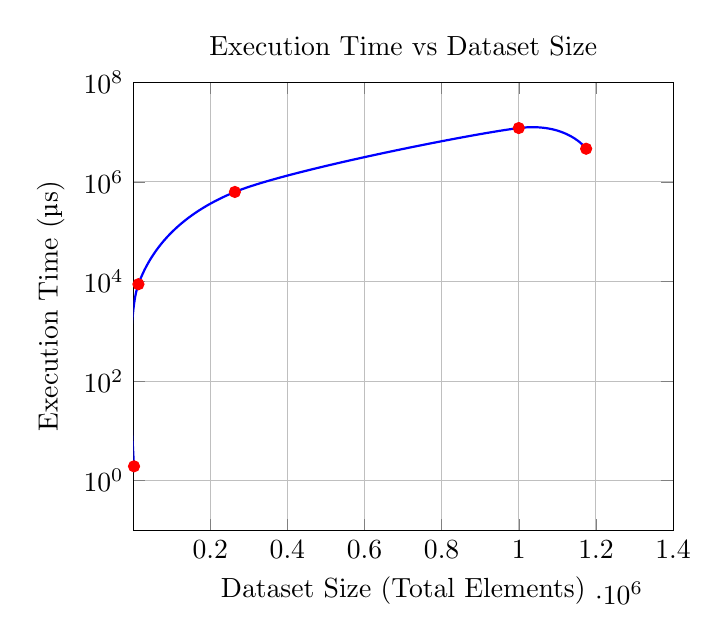
\begin{tikzpicture}
        \begin{axis}[
            ymode=log, % Logarithmic scale for better visualization
            xlabel={Dataset Size (Total Elements)},
            ylabel={Execution Time (µs)},
            title={Execution Time vs Dataset Size},
            xmin=1000, xmax=1400000, % Adjust X-axis limits
            ymin=0.1, ymax=1e8, % Adjust Y-axis limits
            grid=major
        ]
            % Add smooth curve fitting the points
            \addplot[smooth, thick, blue] coordinates {
                (2500, 1.941)
                (13915, 8836.388)
                (264000, 625483.670)
                (1000000, 12000000)
                (1174602, 4612799)
            };
            
            % Add actual data points
            \addplot[
                only marks,
                mark=*,
                red
            ] coordinates {
                (2500, 1.943)
                (13915, 8803.383)
                (264000, 625483.670)
                (1000000, 12000000)
                (1174602, 4612799)
            };
        \end{axis}
    \end{tikzpicture}
    
\subsection{Testing Dataset Details}
The following are the detailed results for the testing dataset:
\begin{lstlisting}[caption=Testing Dataset Execution Details, style=customc]
Running "scalar_naive" implementation:
* Invoking the implementation 100 times .... Finished
* Verifying results .... Success
* Running statistics:
    + Starting statistics run number #1:
    - Standard deviation = 161
    - Average = 1977
    - Number of active elements = 100
    - Number of masked-off = 2
    + Starting statistics run number #2:
    - Standard deviation = 68
    - Average = 1956
    - Number of active elements = 98
    - Number of masked-off = 3
    + Starting statistics run number #3:
    - Standard deviation = 8
    - Average = 1944
    - Number of active elements = 95
    - Number of masked-off = 2
    + Starting statistics run number #4:
    - Standard deviation = 4
    - Average = 1943
    - Number of active elements = 93
    - Number of masked-off = 0
* Runtimes (MATCHING):  1943 ns
\end{lstlisting}

\subsection{Small Dataset Details}
The following are the detailed results for the small dataset:
\begin{lstlisting}[caption=Small Dataset Execution Details, style=customc]
Running "scalar_naive" implementation:
* Invoking the implementation 100 times .... Finished
* Verifying results .... Success
* Running statistics:
    + Starting statistics run number #1:
    - Standard deviation = 1053204
    - Average = 8803383
    - Number of active elements = 100
    - Number of masked-off = 0
* Runtimes (MATCHING):  8803383 ns
\end{lstlisting}


\subsection{Medium Dataset Details}
The following are the detailed results for the medium dataset:
\begin{lstlisting}[caption=Medium Dataset Execution Details, style=customc]
Running "scalar_naive" implementation:
* Invoking the implementation 100 times .... Finished
* Verifying results .... Success
* Running statistics:
    + Starting statistics run number #1:
    - Standard deviation = 496743
    - Average = 625518214
    - Number of active elements = 100
    - Number of masked-off = 2
    + Starting statistics run number #2:
    - Standard deviation = 232254
    - Average = 625516811
    - Number of active elements = 98
    - Number of masked-off = 2
    + Starting statistics run number #3:
    - Standard deviation = 177534
    - Average = 625494911
    - Number of active elements = 96
    - Number of masked-off = 1
    + Starting statistics run number #4:
    - Standard deviation = 169556
    - Average = 625489228
    - Number of active elements = 95
    - Number of masked-off = 1
    + Starting statistics run number #5:
    - Standard deviation = 161620
    - Average = 625483670
    - Number of active elements = 94
    - Number of masked-off = 0
* Runtimes (MATCHING):  625483670 ns
\end{lstlisting}

\subsection{Large Dataset Details}
The following are the detailed results for the large dataset:
\begin{lstlisting}[caption=Large Dataset Execution Details, style=customc]
Running "scalar_naive" implementation:
* Invoking the implementation 100 times .... Finished
* Verifying results .... Success
* Running statistics:
    + Starting statistics run number #1:
    - Standard deviation = 4866044
    - Average = 4613444543
    - Number of active elements = 100
    - Number of masked-off = 2
    + Starting statistics run number #2:
    - Standard deviation = 2936481
    - Average = 4612904698
    - Number of active elements = 98
    - Number of masked-off = 1
    + Starting statistics run number #3:
    - Standard deviation = 2763573
    - Average = 4612799988
    - Number of active elements = 97
    - Number of masked-off = 0
* Runtimes (MATCHING):  4612799988 ns
\end{lstlisting}


\section{Conclusion}
This report documented the implementation and evaluation of the mmult benchmark. The naïve approach demonstrated significant inefficiencies, highlighting the need for optimizations such as loop tiling, vectorization, and parallelization.

\section{References}
\begin{enumerate}
    \item GNU Make Manual: \url{https://www.gnu.org/software/make/manual/make.html}
    \item IEEE POSIX Standard: \url{https://ieeexplore.ieee.org/servlet/opac?punumber=6880749}
    \item YABMS Original Repository: \url{https://github.com/hawajkm/YABMS}
    \item YABMS Forked Repository: \url{https://github.com/mohammed0x00/YABMS}
\end{enumerate}

\end{document}
